\documentclass[12pt]{article}
\usepackage{geometry}                % See geometry.pdf to learn the layout options. There are lots.
\geometry{letterpaper}                   % ... or a4paper or a5paper or ... 
%\geometry{landscape}                % Activate for for rotated page geometry
\usepackage[parfill]{parskip}    % Activate to begin paragraphs with an empty line rather than an indent
\usepackage{graphicx}
\usepackage{amssymb}
\usepackage{subfig}
\usepackage{pstricks,pst-node,pst-tree}



\title{Breakpoints for farm field runoff}
\author{Wesley Brooks}
\date{}                                           % Activate to display a given date or no date

\usepackage{Sweave}
\begin{document}
\setkeys{Gin}{width=0.9\textwidth}    %make figures a bit wider than the Sweave default.
\maketitle






The following is the R code used to produce a piecewise regression model:

\begin{Schunk}
\begin{Sinput}
> piecewise <- function(th, x, y) { # 
+         X <- cbind( ifelse(x>=th, 1, 0), x, pmax(0, x-th) )
+         fit = lsfit(X, y) #actually fit the model
+         
+         #Counts how many observations lie above and below the breakpoint
+         upper = as.logical( ifelse(x-th>=0, 1, 0) )
+         n_upper = sum(upper)
+         n_lower = dim(X)[1] - n_upper
+         
+         #Sum of squared residuals on either side of the breakpoint
+         ssr_upper = sum( fit$resid[upper]**2 )
+         ssr_lower = sum( fit$resid[!upper]**2 )
+         
+         #Return the residual standard error:
+         return( n_lower*sqrt(ssr_lower/(n_lower-2)) 
+             + n_upper*sqrt(ssr_upper/(n_upper-2)) ) }
\end{Sinput}
\end{Schunk}


\vspace{10mm}
We identify the best breakpoint by using R's optimize function to minimize the residual standard error:

\begin{Schunk}
\begin{Sinput}
> soil_moisture_limits = c(33, 43) #set the limits
> optimize(piecewise, soil_moisture_limits, x=data$sm, y=data$rc)$minimum
\end{Sinput}
\end{Schunk}



\vspace{10mm}
First, let us do the soil moisture breakpoint analysis. The breakpoints at each farm individually, and for all farms in aggregate are:


\begin{Schunk}
\begin{Soutput}
Kp: 35
P: 35
Pf: 36
R: 36
S: 40
\end{Soutput}
\begin{Soutput}
aggregate: 35
\end{Soutput}
\end{Schunk}



\begin{figure}
    \begin{center}
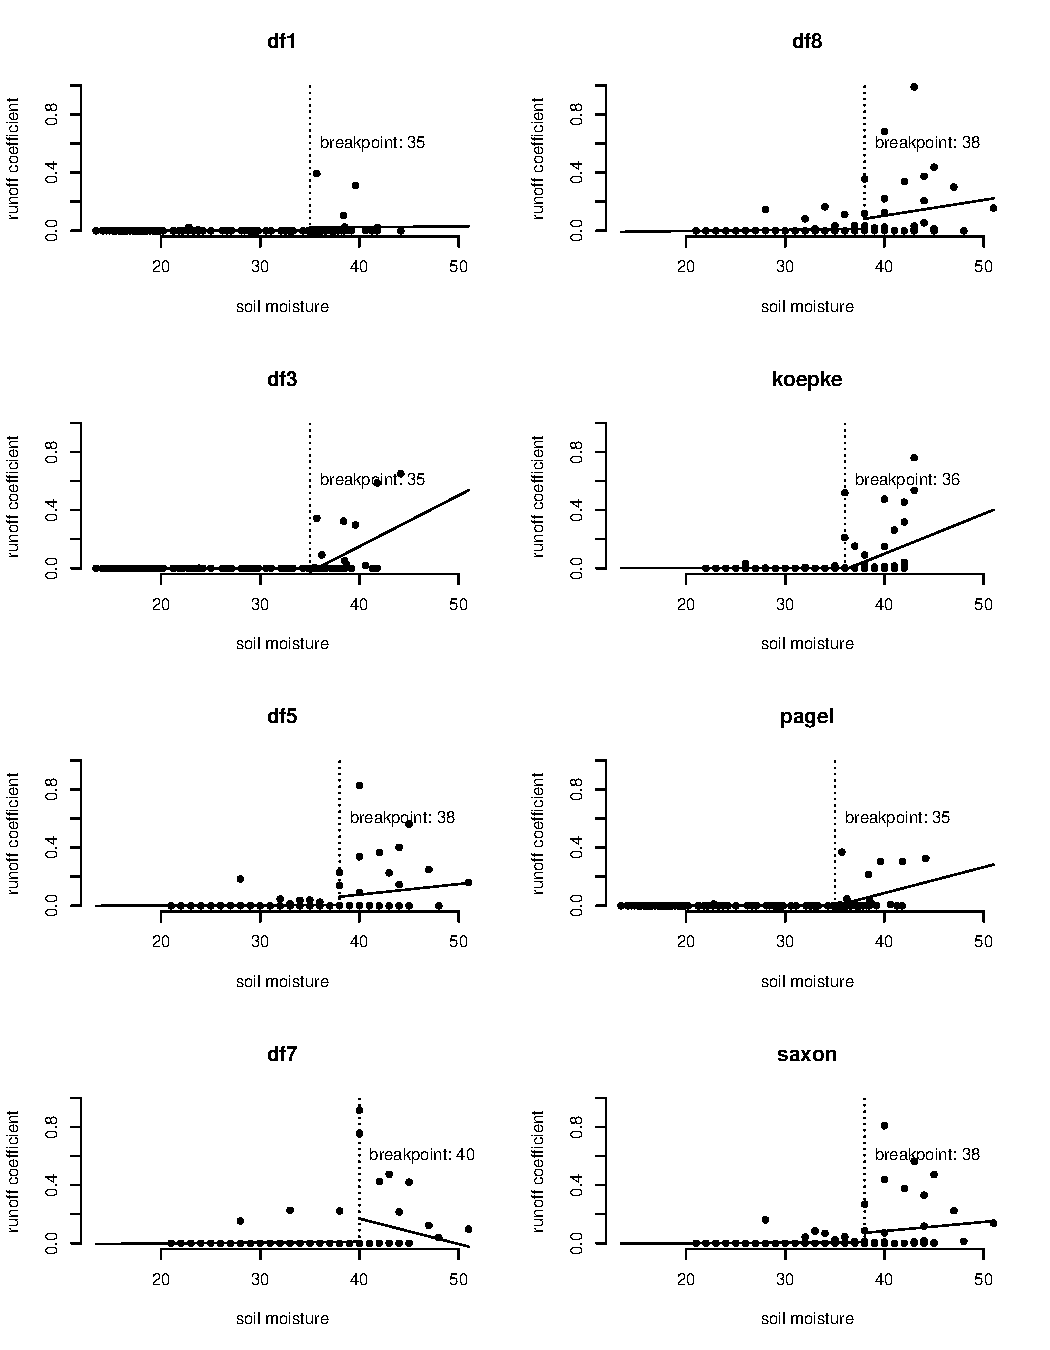
\includegraphics{runoff-sm}
    \end{center}
    \caption{caption.\label{sm}}
\end{figure}


\vspace{10mm}
Now get the I30 breakpoints:

\begin{Schunk}
\begin{Soutput}
Kp: 0.5
P: 0.8
Pf: 0.7
R: 0.6
S: 0.9
\end{Soutput}
\begin{Soutput}
aggregate: 0.6
\end{Soutput}
\end{Schunk}


\vspace{10mm}
When we put the events in bins based on their antecedent soil moisture (SM: high, medium, and low), the following are the I30 breakpoints (inches of rain per hour):

\begin{Schunk}
\begin{Soutput}
-Inf <= SM < 30: 1.7
30 <= SM < 35: 0.5
35 <= SM < Inf: 0.8
\end{Soutput}
\end{Schunk}



\begin{figure}
    \begin{center}
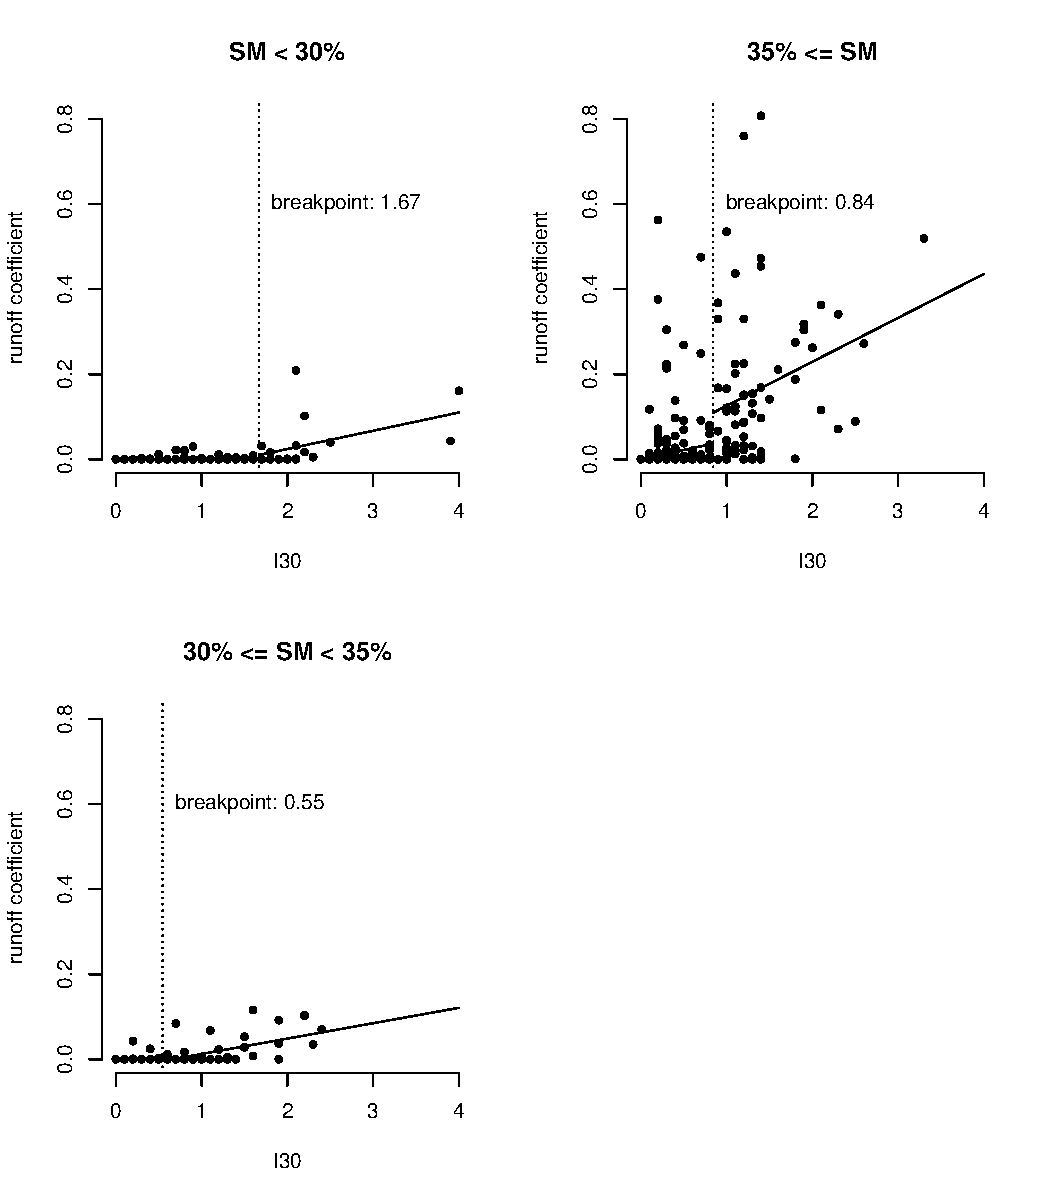
\includegraphics{runoff-I30_binned}
    \end{center}
    \caption{caption.\label{I30_binned}}
\end{figure}


\vspace{10mm}
When we put the events in bins based on their antecedent soil moisture (SM: high, medium, and low), the following are the rain depth breakpoints (inches of rain):

\begin{Schunk}
\begin{Soutput}
-Inf <= SM < 30: 1.3
30 <= SM < 35: 0.94
35 <= SM < Inf: 0.45
\end{Soutput}
\end{Schunk}





\begin{figure}
    \begin{center}
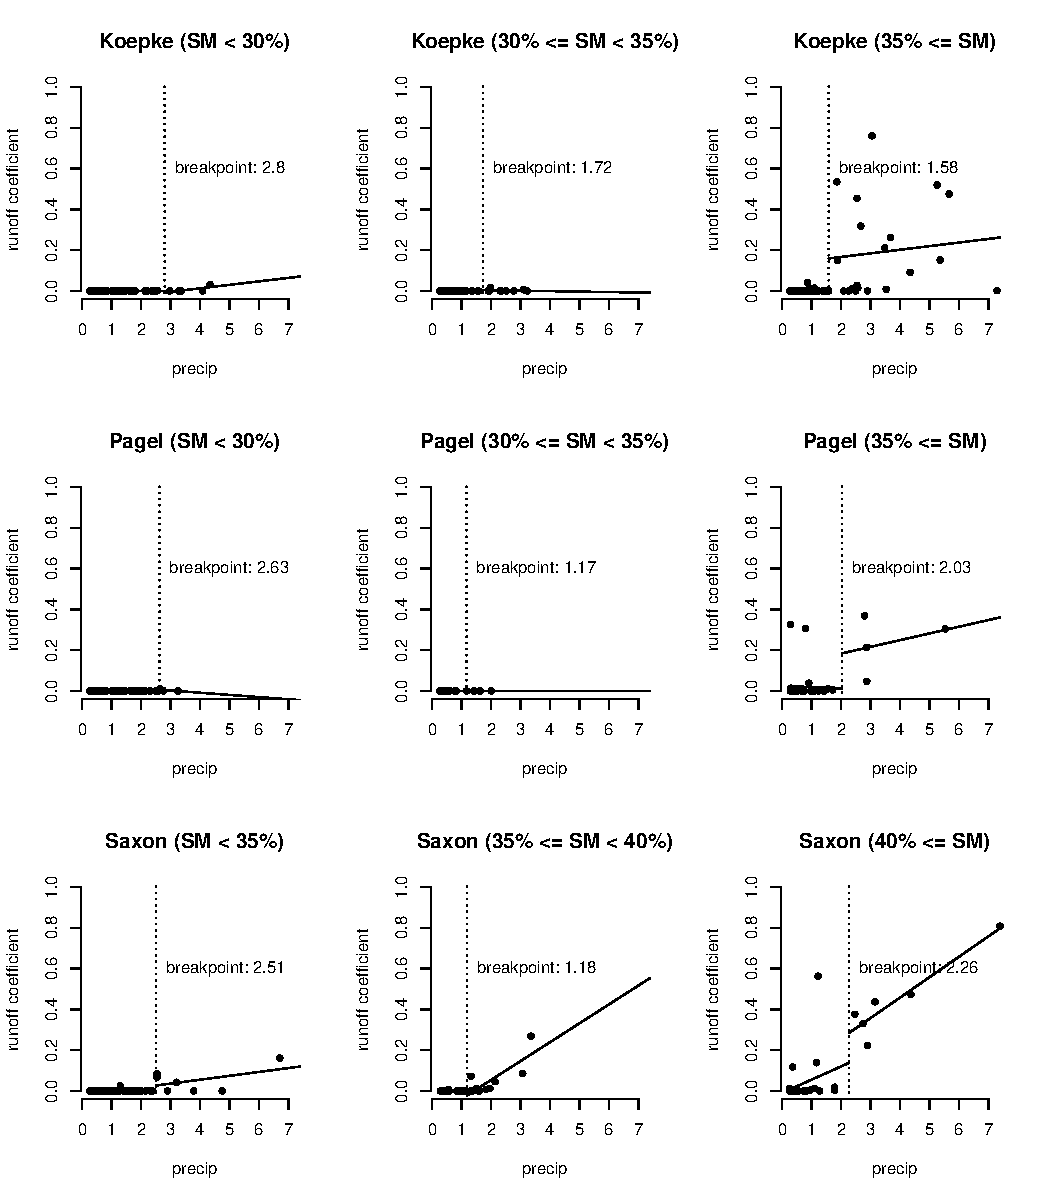
\includegraphics{runoff-precip_binned}
    \end{center}
    \caption{caption.\label{precip_binned}}
\end{figure}


\end{document}
